根据上一节中的信息,您现在可以使用LLVM库创建自己的项目。下面几节介绍一种名为Tiny的小型语言,这个项目将称为tinylang。这里定义了这样一个项目的结构。尽管本节中的工具只是一个Hello, world应用程序,但它的结构具有真实的编译器所需的所有部分。\par

\hspace*{\fill} \par %插入空行
\textbf{创建目录结构}

第一个问题是,tinylang项目是否应该与LLVM一起构建(就像clang一样),还是应该是一个只使用LLVM库的独立项目。前一种情况下,还需要决定在哪里创建项目。\par

首先假设tinylang应该与LLVM一起构建。在哪里放置项目有不同的选择。第一种解决方案是在llvm-projects目录中为项目创建一个子目录。此目录中的所有项目都将作为构建LLVM的一部分使用并构建。在并行项目布局创建之前,这是标准的构建方式,例如:clang。\par

第二种选择是将tinylang项目放在顶级目录中。因为它不是一个正式的LLVM项目,所以CMake脚本不知道它。当运行cmake时,你需要指定-DLLVM \underline{~}ENABLE\underline{~}PROJECTS=tinylang,以便在构建中包含项目。\par

第三种选择是将项目目录放在其他地方,即llvm-project目录之外。当然,需要告诉CMake关于这个位置。例如,如果位置是/src/tinylang,那么需要指定-DLLVM \underline{~}ENABLE\underline{~}PROJECTS=tinylang -DLLVM \underline{~}EXTERNAL\underline{~} tinylang \underline{~}SOURCE\underline{~}DIR=/src/tinylang。\par

如果您希望将项目作为独立项目构建,那么需要找到LLVM库。这是在CMakeLists.txt文件中完成的,本节稍后将讨论这个文件。\par

在了解了可能的选择后,哪一个最好呢?使您的项目成为LLVM源代码树的一部分有点不灵活。只要您不打算将您的项目添加到顶级项目列表中,我建议使用一个单独的目录。可以在GitHub或类似的服务上维护你的项目,而不用担心如何与LLVM项目同步。正如前面所示,您仍然可以与其他LLVM项目一起构建它。\par

让我们用一个非常简单的库和应用程序创建一个项目。第一步是创建目录布局。选择一个你方便的地方。在下面的步骤中,我假设它位于克隆llvm-project目录的同一个目录中。使用mkdir(Unix)或md(Windows)创建以下目录:\par

\hspace*{\fill} \par %插入空行
\begin{center}
	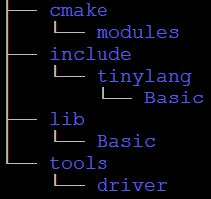
\includegraphics{content/1/chapter2/images/2.jpg}\\
	图2.2 – 项目所需的目录
\end{center}

接下来,我们将构建描述和源文件放在这些目录中。\par

\hspace*{\fill} \par %插入空行
\textbf{添加CMake文件}

您应该从上一节中确认了代码的基本结构。在tinylang目录中,按照以下步骤创建一个名为CMakeLists.txt的文件:\par

\begin{enumerate}
	\item 该文件首先使用cmake\underline{~}minimum\underline{~}required()来声明CMake的最低必需版本:
	\begin{tcolorbox}[colback=white,colframe=black]
		cmake\underline{~}minimum\underline{~}required(VERSION 3.13.4)
	\end{tcolorbox}
 	\item 下一个语句是if()。如果条件为真,那么项目将独立构建,并且需要一些额外的设置。该条件使用两个变量,CMAKE\underline{~}SOURCE\underline{~}DIR和CMAKE\underline{~}CURRENT\underline{~}SOURCE\underline{~}DIR。CMAKE\underline{~}SOURC\allowbreak E\underline{~}DIR变量是在CMAKE命令行中给出的顶层源目录。正如在关于目录布局的讨论中所看到的,每个带有源文件的目录都有一个CMakeLists.txt文件。CMakeLists.txt文件所位于的当前文件夹记录在CMake\underline{~}CURRENT\underline{~}SOURCE\underline{~}DIR变量中。如果两个变量具有相同的字符串值,那么项目将独立构建。否则,CMAKE\underline{~}SOURCE\underline{~}DIR将是llvm目录:
 	\begin{tcolorbox}[colback=white,colframe=black]
 		if(CMAKE\underline{~}SOURCE\underline{~}DIR STREQUAL CMAKE\underline{~}CURRENT\underline{~}SOURCE\underline{~}DIR)
 	\end{tcolorbox}
 	独立的设置很简单,每个CMake项目都需要一个名称。这里,我们将它设置为Tinylang:
 	\begin{tcolorbox}[colback=white,colframe=black]
 		project(Tinylang)
 	\end{tcolorbox}
 	\item 搜索LLVM包,并将LLVM目录添加到CMake模块路径中:
 	\begin{tcolorbox}[colback=white,colframe=black]
 		find\underline{~}package(LLVM REQUIRED HINTS \\
 		"\${LLVM\underline{~}CMAKE\underline{~}PATH}") \\
 		list(APPEND CMAKE\underline{~}MODULE\underline{~}PATH \${LLVM\underline{~}DIR})
 	\end{tcolorbox}
 	\item 然后,包含了LLVM提供的另外三个CMake模块。只有当使用Visual Studio作为构建编译器,并设置正确的运行时库,再次链接时才需要第一个。另外两个模块添加LLVM使用的宏,并根据提供的选项配置构建:
 	\begin{tcolorbox}[colback=white,colframe=black]
 		include(ChooseMSVCCRT) \\
 		include(AddLLVM) \\
 		include(HandleLLVMOptions)
 	\end{tcolorbox}
 	\item 接下来,将LLVM头文件的路径添加到include搜索路径中。新增两个目录。添加了构建目录中的include目录,因为这里保存了自动生成的文件。另一个include目录位于源目录中:
 	\begin{tcolorbox}[colback=white,colframe=black]
 		include\underline{~}directories("\${LLVM\underline{~}BINARY\underline{~}DIR}/include" \\
 		"\${LLVM\underline{~}INCLUDE\underline{~}DIR}")
 	\end{tcolorbox}
 	\item 使用link\underline{~}directories(),LLVM库的路径添加到链接器中:
 	\begin{tcolorbox}[colback=white,colframe=black]
 		link\underline{~}directories("\${LLVM\underline{~}LIBRARY\underline{~}DIR}")
 	\end{tcolorbox}
 	\item 作为最后一步,设置一个标志来表示项目是独立构建的:
 	\begin{tcolorbox}[colback=white,colframe=black]
 		set(TINYLANG\underline{~}BUILT\underline{~}STANDALONE 1)
      endif()
 	\end{tcolorbox}
 	\item 现在遵循常见的设置。将cmake/modules目录添加到CMake模块搜索路径中。这允许添加自己的CMake模块:
 	\begin{tcolorbox}[colback=white,colframe=black]
      list(APPEND CMAKE\underline{~}MODULE\underline{~}PATH \\
 		"\${CMAKE\underline{~}CURRENT\underline{~}SOURCE\underline{~}DIR}/cmake/modules")
 	\end{tcolorbox}
 	\item 接下来,检查用户是否正在执行超出构建树的构建。与LLVM一样,我们要求用户使用一个单独的目录来构建项目:
 	\begin{tcolorbox}[colback=white,colframe=black]
 		if(CMAKE\underline{~}SOURCE\underline{~}DIR STREQUAL CMAKE\underline{~}BINARY\underline{~}DIR AND NOT MSVC\underline{~}IDE) \\
   		  message(FATAL\underline{~}ERROR "In-source builds are not allowed.") \\
 		endif()
 	\end{tcolorbox}
 	\item tinylang的版本号通过configure\underline{~}file()命令写到生成的文件中。版本号取自TINYLANG\underline{~}VER\allowbreak SION\underline{~}STRING 变量。configure\underline{~}file()命令读取一个输入文件,用CMake变量的当前值替换它们,并写入一个输出文件。请注意,输入文件是从源目录读取的,并写入构建目录:
 	\begin{tcolorbox}[colback=white,colframe=black]
 		set(TINYLANG\underline{~}VERSION\underline{~}STRING "0.1") \\
 		configure\underline{~}file(\${CMAKE\underline{~}CURRENT\underline{~}SOURCE\underline{~}DIR}/include/ \\
 		tinylang/Basic/Version.inc.in \\
 		  \${CMAKE\underline{~}CURRENT\underline{~}BINARY\underline{~}DIR}/include/tinylang/Basic/Version.inc)
 	\end{tcolorbox}
 	\item 接下来,将包含另一个CMake模块。AddTinylang模块有一些辅助功能:
 	\begin{tcolorbox}[colback=white,colframe=black]
 		include(AddTinylang)
 	\end{tcolorbox}
 	\item 接下来是另一个include\underline{~}directories()语句。将把我们自己的include目录添加到搜索路径的开头。在独立版本中,添加了两个目录:
 	\begin{tcolorbox}[colback=white,colframe=black]
 		include\underline{~}directories(BEFORE \\
 		\${CMAKE\underline{~}CURRENT\underline{~}BINARY\underline{~}DIR}/include \\
 		\${CMAKE\underline{~}CURRENT\underline{~}SOURCE\underline{~}DIR}/include \\
 		)
 	\end{tcolorbox}
 	\item 在文件的末尾,在lib和tools目录其中找到CMakeLists.txt文件,这是连接目录的基本机制。这个示例应用程序只有lib和tools目录下的源文件,因此不需要其他文件。更复杂的项目将添加更多的目录,例如:单元测试:
 	\begin{tcolorbox}[colback=white,colframe=black]
 		add\underline{~}subdirectory(lib) \\
 		add\underline{~}subdirectory(tools)
 	\end{tcolorbox}
\end{enumerate}

这就是您项目的描述。\par

AddTinylang.make协助模块位于cmake/modules目录下。有以下内容:\par

\begin{lstlisting}[caption={}]
macro(add_tinylang_subdirectory name)
  add_llvm_subdirectory(TINYLANG TOOL ${name})
endmacro()

macro(add_tinylang_library name)
  if(BUILD_SHARED_LIBS)
    set(LIBTYPE SHARED)
  else()
    set(LIBTYPE STATIC)
  endif()
  
  llvm_add_library(${name} ${LIBTYPE} ${ARGN})
  if(TARGET ${name})
    target_link_libraries(${name} INTERFACE
      ${LLVM_COMMON_LIBS})
    install(TARGETS ${name}
      COMPONENT ${name}
      LIBRARY DESTINATION lib${LLVM_LIBDIR_SUFFIX}
      ARCHIVE DESTINATION lib${LLVM_LIBDIR_SUFFIX}
      RUNTIME DESTINATION bin)
  else()
    add_custom_target(${name})
  endif()
endmacro()

macro(add_tinylang_executable name)
  add_llvm_executable(${name} ${ARGN} )
endmacro()

macro(add_tinylang_tool name)
  add_tinylang_executable(${name} ${ARGN})
  install(TARGETS ${name}
    RUNTIME DESTINATION bin
    COMPONENT ${name})
endmacro()
\end{lstlisting}

通过包含该模块,可以使用add\underline{~}tinylang\underline{~}subdirectory()、add\underline{~}tinylang\underline{~}library()、add\underline{~}tinylang\underline{~}exe\allowbreak cutable()和add\underline{~}tinylang\underline{~}tool()函数。这些是LLVM(在AddLLVM模块中)提供的函数包装器。tinylang\underline{~}subdirectory()为构建添加了一个新的源目录。此外,还添加了一个新的CMake选项。使用此选项,用户可以控制是否应该编译目录的内容。使用add\underline{~}tinylang\underline{~}library(),可以定义库并安装。Add \underline{~}tinylang\underline{~}executable()定义了可执行文件,Add \underline{~}tinylang\underline{~}tool()定义了同样安装的可执行文件。\par

在lib目录中,即使没有源代码,也需要CMakeLists.txt文件,必须包含这个项目库的源目录。打开文本编辑器,并将以下内容保存在文件中:\par

\begin{tcolorbox}[colback=white,colframe=black]
add\underline{~}subdirectory(Basic)
\end{tcolorbox}

大型项目将创建几个库,源代码将放在lib的子目录中。每个目录都必须添加到CMakeLists.txt文件中。我们的小项目只有一个名为Basic的库,所以只需要一行代码。\par

Basic库只有一个源文件Version.cpp。这个目录中的CMakeLists.txt文件同样简单:\par

\begin{tcolorbox}[colback=white,colframe=black]
add\underline{~}tinylang\underline{~}library(tinylangBasic \\
Version.cpp \\
)
\end{tcolorbox}

定义了一个名为tinylangBasic的新库,并将编译后的Version.cpp添加到这个库中。LLVM选项可以控制这是一个动态库还是静态库。默认情况下,会创建静态库。\par

在tools目录中重复相同的步骤。这个文件夹中的CMakeLists.txt文件几乎和lib目录中一样简单:\par

\begin{tcolorbox}[colback=white,colframe=black]
create\underline{~}subdirectory\underline{~}options(TINYLANG TOOL) \\
add\underline{~}tinylang\underline{~}subdirectory(driver)
\end{tcolorbox}

首先,定义了一个CMake选项来控制该目录的内容是否编译。然后添加子目录driver,这一次使用我们自己的模块函数。同样,这让我们可以控制这个目录是否包含在编译中。\par

驱动程序目录包含应用程序的源码driver.cpp。这个目录中的CMakeLists.txt文件包含了编译和链接这个应用程序的所有步骤:\par

\begin{tcolorbox}[colback=white,colframe=black]
set(LLVM\underline{~}LINK\underline{~}COMPONENTS\\
Support\\
)\\
\\
add\underline{~}tinylang\underline{~}tool(tinylang\\
Driver.cpp\\
) \\

target\underline{~}link\underline{~}libraries(tinylang \\
PRIVATE\\
tinylangBasic\\
)
\end{tcolorbox}

首先,LLVM\underline{~}LINK\underline{~}COMPONENTS变量设置为需要链接的LLVM组件列表(LLVM组件是一个或多个库的集合)。显然,这取决于工具实现的功能。这里,我们只需要Support组件。\par

使用add\underline{~}tinylang\underline{~}tool()定义了可安装应用程序。名称是tinylang,唯一的源文件是Driver.cpp。要链接到自己的库,必须使用target\underline{~}link\underline{~}libraries()来指定。这里,只需要tinylangBasic。\par

现在,CMake所需的文件已经就绪。接下来,需要添加源文件。\par

\hspace*{\fill} \par %插入空行
\textbf{创建目录结构}

让我们从include/tinylang/Basic目录开始。首先,创建Version.inc.in模板文件,其中包含配置的版本号:\par

\begin{lstlisting}[caption={}]
#define TINYLANG_VERSION_STRING "@TINYLANG_VERSION_STRING@"
\end{lstlisting}

TINYLANG\underline{~}VERSION\underline{~}STRING周围的@符号表示这是一个CMake变量,可以进行内容替换。\par

Version.h头文件声明了一个可获取version字符串的函数:\par

\begin{lstlisting}[caption={}]
#ifndef TINYLANG_BASIC_VERSION_H
#define TINYLANG_BASIC_VERSION_H

#include "tinylang/Basic/Version.inc"
#include <string>

namespace tinylang {
	std::string getTinylangVersion();
}

#endif
\end{lstlisting}

这个函数的实现在lib/Basic/Version.cpp文件中。同样很简单:\par

\begin{lstlisting}[caption={}]
#include "tinylang/Basic/Version.h"

std::string tinylang::getTinylangVersion() {
	return TINYLANG_VERSION_STRING;
}
\end{lstlisting}

最后,在tools/driver/Driver.cpp文件中有应用程序的源代码:\par

\begin{lstlisting}[caption={}]
#include "llvm/Support/InitLLVM.h"
#include "llvm/Support/raw_ostream.h"
#include "tinylang/Basic/Version.h"

int main(int argc_, const char **argv_) {
	llvm::InitLLVM X(argc_, argv_);
	llvm::outs() << "Hello, I am Tinylang "
	<< tinylang::getTinylangVersion()
	<< "\n";
}
\end{lstlisting}

尽管只是一个友好的工具,但源码使用了典型的LLVM功能。调用llvm::InitLLVM()执行一些基本的初始化。在Windows上,参数被转换为Unicode,以便对命令行解析进行统一处理。在应用程序崩溃的情况下(希望不太可能),将安装一个打印堆栈跟踪处理程序。它输出调用层次结构,从发生崩溃的函数开始。要查看真正的函数名而不是十六进制地址,必须提供调试符号。\par

LLVM不使用C++标准库的iostream类,它有自己的实现。llvm::outs()是输出流,在这里用来向用户发送消息。\par

\hspace*{\fill} \par %插入空行
\textbf{编译tinylang应用程序}

现在第一个应用程序的所有文件都已就绪,可以编译该应用程序了。概括一下,应该有以下目录和文件:\par

\hspace*{\fill} \par %插入空行
\begin{center}
	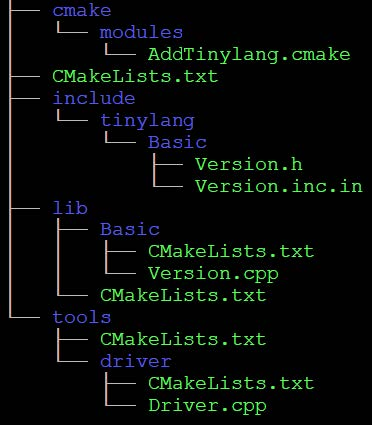
\includegraphics{content/1/chapter2/images/3.jpg}\\
	图2.3 – tinylang项目的所有目录和文件
\end{center}

如前所述,有几种方法可以构建tinylang。下面是如何将tinylang构建为LLVM的一部分:\par

\begin{enumerate}
\item 使用下面的命令进入构建目录:
	\begin{tcolorbox}[colback=white,colframe=black]
	\$ cd build
	\end{tcolorbox}

\item 执行如下CMake命令。
	\begin{tcolorbox}[colback=white,colframe=black]
	\$ cmake -G Ninja -DCMAKE\underline{~}BUILD\underline{~}TYPE=Release $\setminus$ \\
	-DLLVM\underline{~}EXTERNAL\underline{~}PROJECTS=tinylang $\setminus$ \\
	-DLLVM\underline{~}EXTERNAL\underline{~}TINYLANG\underline{~}SOURCE\underline{~}DIR=../tinylang $\setminus$ \\
	-DCMAKE\underline{~}INSTALL\underline{~}PREFIX=../llvm-12 $\setminus$ \\
	../llvm-project/llvm
	\end{tcolorbox}
	通过这个命令,CMake为Ninja(-G Ninja)生成构建文件。构建类型设置为Release,从而生成优化的二进制文件(-DCMAKE\underline{~}BUILD\underline{~}TYPE=Release)。Tinylang作为一个外部项目与LLVM(-DLLVM\underline{~}EXTERNAL\underline{~}PROJECTS=Tinylang)一起构建,源代码位于与构建目录平行的目录中(-DLLVM\underline{~} EXTERNAL\underline{~}TINYLANG\underline{~}SOURCE\underline{~}DIR=../Tinylang)。还提供了构建二进制文件的目标目录(-DCMAKE\underline{~}INSTALL\underline{~}PREFIX=../llvm-12)。最后一个参数指定LLVM项目目录(../llvm-project/llvm)。
	
\item 现在,进行构建和安装:
\begin{tcolorbox}[colback=white,colframe=black]
\$ ninja \\
\$ ninja install
\end{tcolorbox}

\item 构建安装完成后,../llvm-12目录会包含LLVM和tinylang二进制文件。请检查这些应用是否可以运行:
\begin{tcolorbox}[colback=white,colframe=black]
\$ ../llvm-12/bin/tinylang
\end{tcolorbox}

\item 您应该看到一些友好的消息。请同时检查Basic库是否安装:
\begin{tcolorbox}[colback=white,colframe=black]
	\$ ls ../llvm-12/lib/libtinylang*
\end{tcolorbox}
这将显示有一个名为libtinylangBasic.a的文件。

\end{enumerate}

当您密切关注LLVM的开发,并且希望尽快了解API的变化时,使用LLVM进行构建非常有用。第一章中,我们检查了LLVM的特定版本。因此,没有看到对LLVM源的修改。\par

这里,只构建一次LLVM,然后使用已编译的LLVM版本,将tinylang作为独立项目进行编译:\par

\begin{enumerate}
	\item 重新开始,再次进入构建目录:
	\begin{tcolorbox}[colback=white,colframe=black]
		\$ cd build
	\end{tcolorbox}
	这一次,CMake仅用于构建LLVM:
	\begin{tcolorbox}[colback=white,colframe=black]
		\$ cmake -G Ninja -DCMAKE\underline{~}BUILD\underline{~}TYPE=Release $\setminus$ \\
		-DCMAKE\underline{~}INSTALL\underline{~}PREFIX=../llvm-12 $\setminus$ \\
		../llvm-project/llvm
	\end{tcolorbox}

	\item 与前面的CMake命令比较,除了tinylang的参数没了,其他都一样。
	
	\item 创建和安装LLVM与Ninja:
	\begin{tcolorbox}[colback=white,colframe=black]
		\$ ninja \\
		\$ ninja install
	\end{tcolorbox}

	\item 现在您已经在llvm-12目录中安装了一个LLVM。接下来,将对tinylang项目进行建成。由于它是一个独立的构建,因此需要一个新的构建目录:
	\begin{tcolorbox}[colback=white,colframe=black]
		\$ cd ..
	\end{tcolorbox}
	
	\item 现在创建一个新的build-tinylang目录。在Unix上,可以使用以下命令:
	\begin{tcolorbox}[colback=white,colframe=black]
		\$ mkdir build-tinylang
	\end{tcolorbox}

	在Windows上,可以使用这个命令:
	\begin{tcolorbox}[colback=white,colframe=black]
		\$ md build-tinylang
	\end{tcolorbox}

	\item 在任意一个操作系统上用以下命令输入新目录:
	\begin{tcolorbox}[colback=white,colframe=black]
		\$ cd build-tinylang
	\end{tcolorbox}
	
	\item 现在运行CMake来创建tinylang的构建文件。唯一的问题是如何发现LLVM,因为CMake不知道LLVM的安装位置。解决方案是指定LLVMConfig.cmake的路径。使用LLVM\underline{~}DIR变量指定该cmake文件所在的文件夹。命令如下:
	\begin{tcolorbox}[colback=white,colframe=black]
		\$ cmake -G Ninja -DCMAKE\underline{~}BUILD\underline{~}TYPE=Release $\setminus$ \\
		-DLLVM\underline{~}DIR=../llvm-12/lib/cmake/llvm $\setminus$ \\
		-DCMAKE\underline{~}INSTALL\underline{~}PREFIX=../tinylang ../tinylang/
	\end{tcolorbox}

	\item 安装目录现在也是分开的。像往常一样,构建和安装如下:
	\begin{tcolorbox}[colback=white,colframe=black]
		\$ ninja \\
		\$ ninja install
	\end{tcolorbox}
	\item 在命令完成后,应该运行../tinylang/bin/tinylang应用程序检查应用程序是否正常。
\end{enumerate}


\hspace*{\fill} \par %插入空行
\textbf{包含LLVM的另一种方法}

如果不想在项目中使用CMake,那么需要找出包含文件和库的位置、要链接的库、使用的构建模式等等。此信息由llvm-config工具提供,该工具位于LLVM安装的bin目录中。假设这个目录包含在shell搜索路径中,可以运行\textit{\$llvm-config}查看所有选项。\par

例如,要让LLVM库链接到支持组件(在前面的示例中使用),可以运行以下命令:\par

\begin{tcolorbox}[colback=white,colframe=black]
	\$ llvm-config –libs support
\end{tcolorbox}

输出是一行带有库名的代码,包括编译器的链接选项,例如-lLLVMSupport 、-lLLVMDemangle。显然,这个工具可以很容易地与您所选择的构建系统进行集成。\par

有了本节所示的项目布局,您就有了一个可扩展到大型项目(如编译器)的结构。下一节将介绍另一个基础只是:如何针对不同的目标体系结构进行交叉编译。\par












